\section{Additional Recommendations}\label{sec:additional}

A small change to the southern portion of the footprint improves overlap with the Euclid footprint and determines negligible changes in science metrics. 
\begin{figure}
\centering
%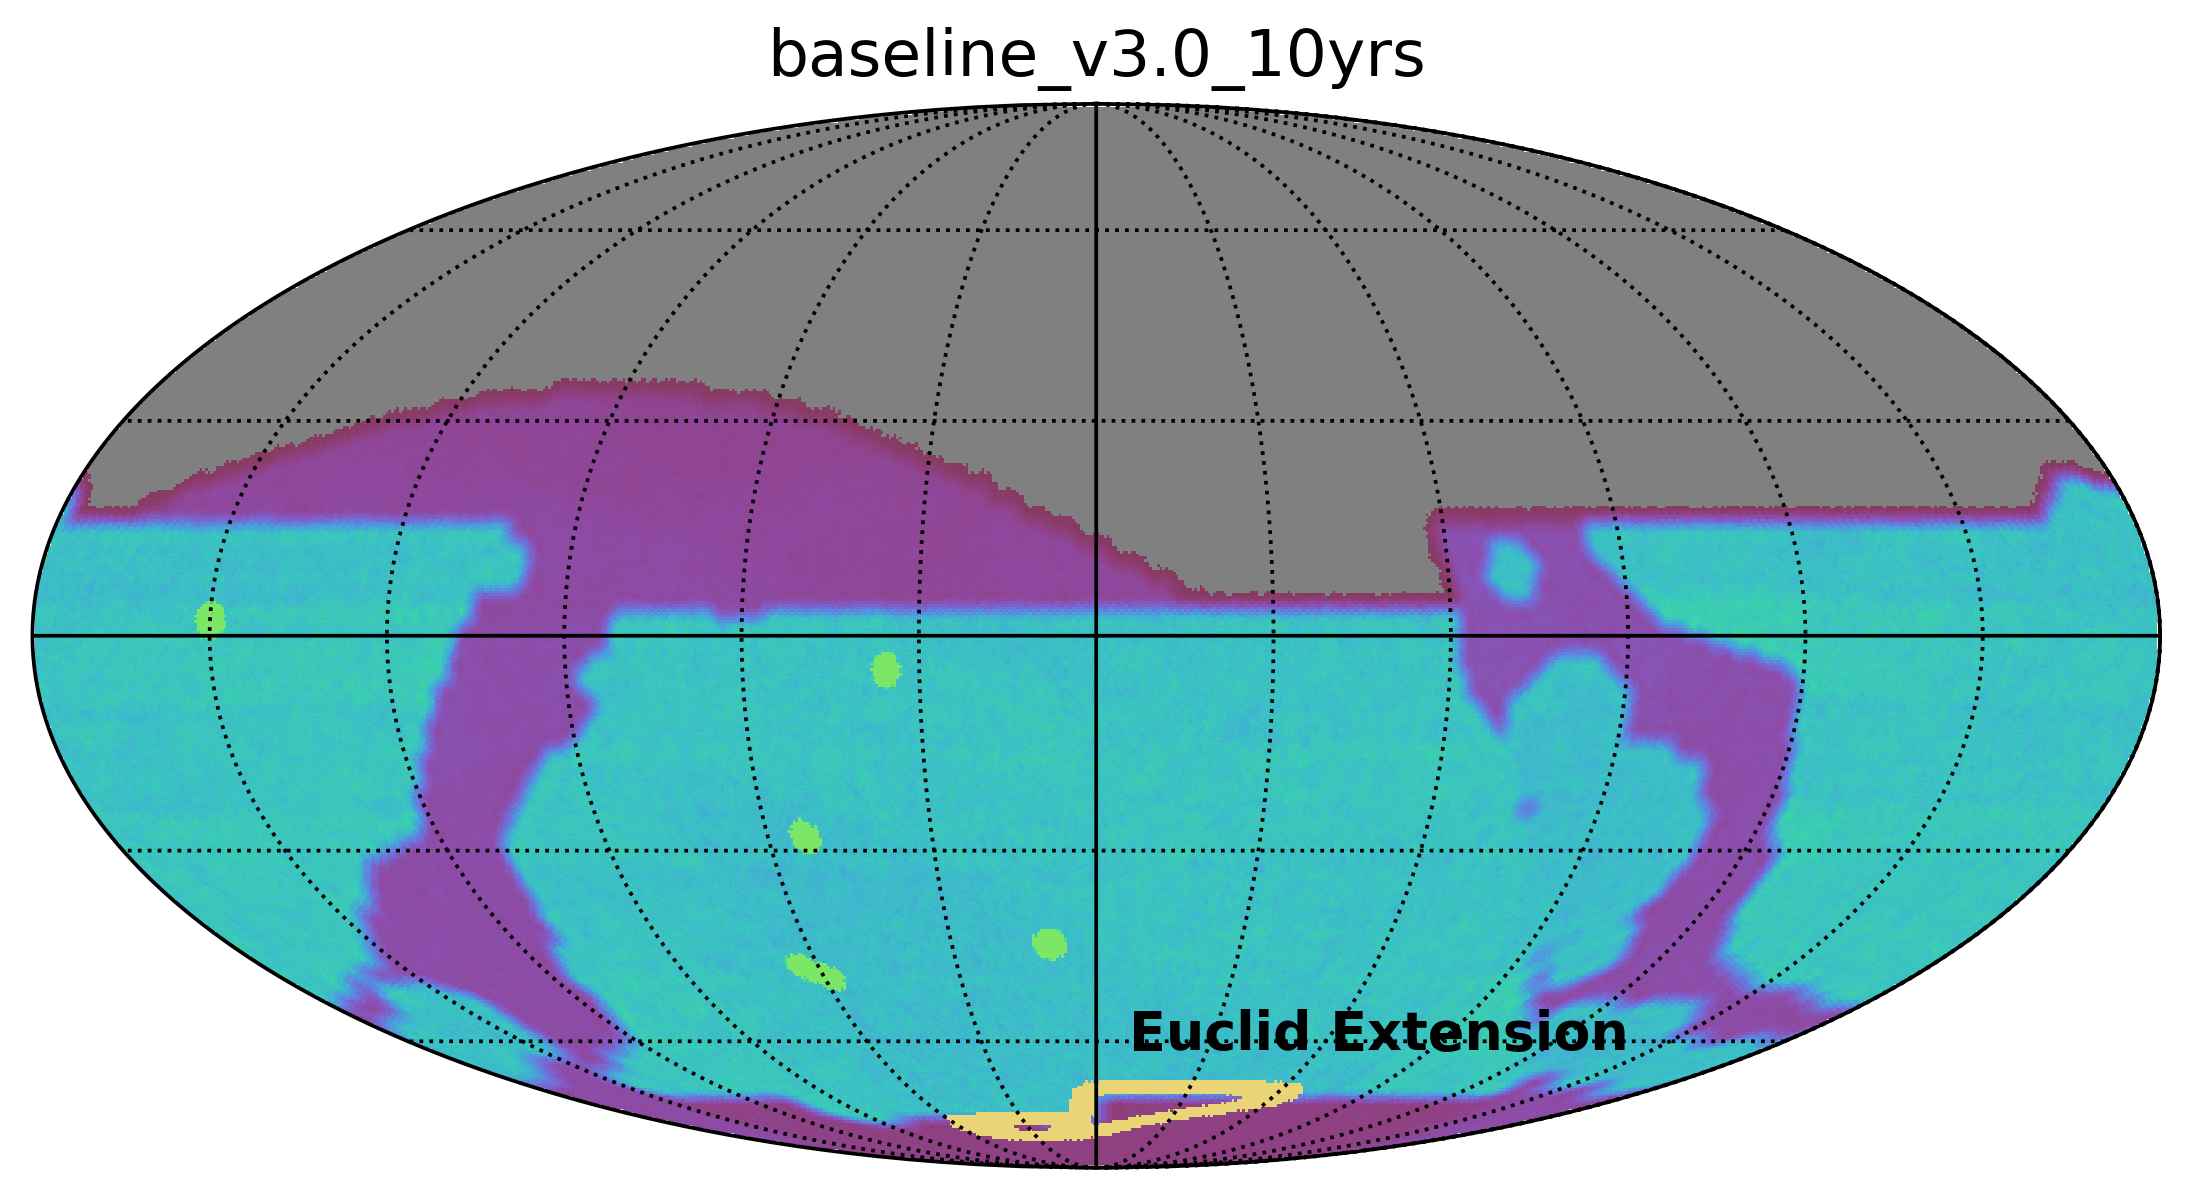
\includegraphics[width=0.45\textwidth]{figures/baseline_v3_0_10yrs_euclid_overlap.pdf}
%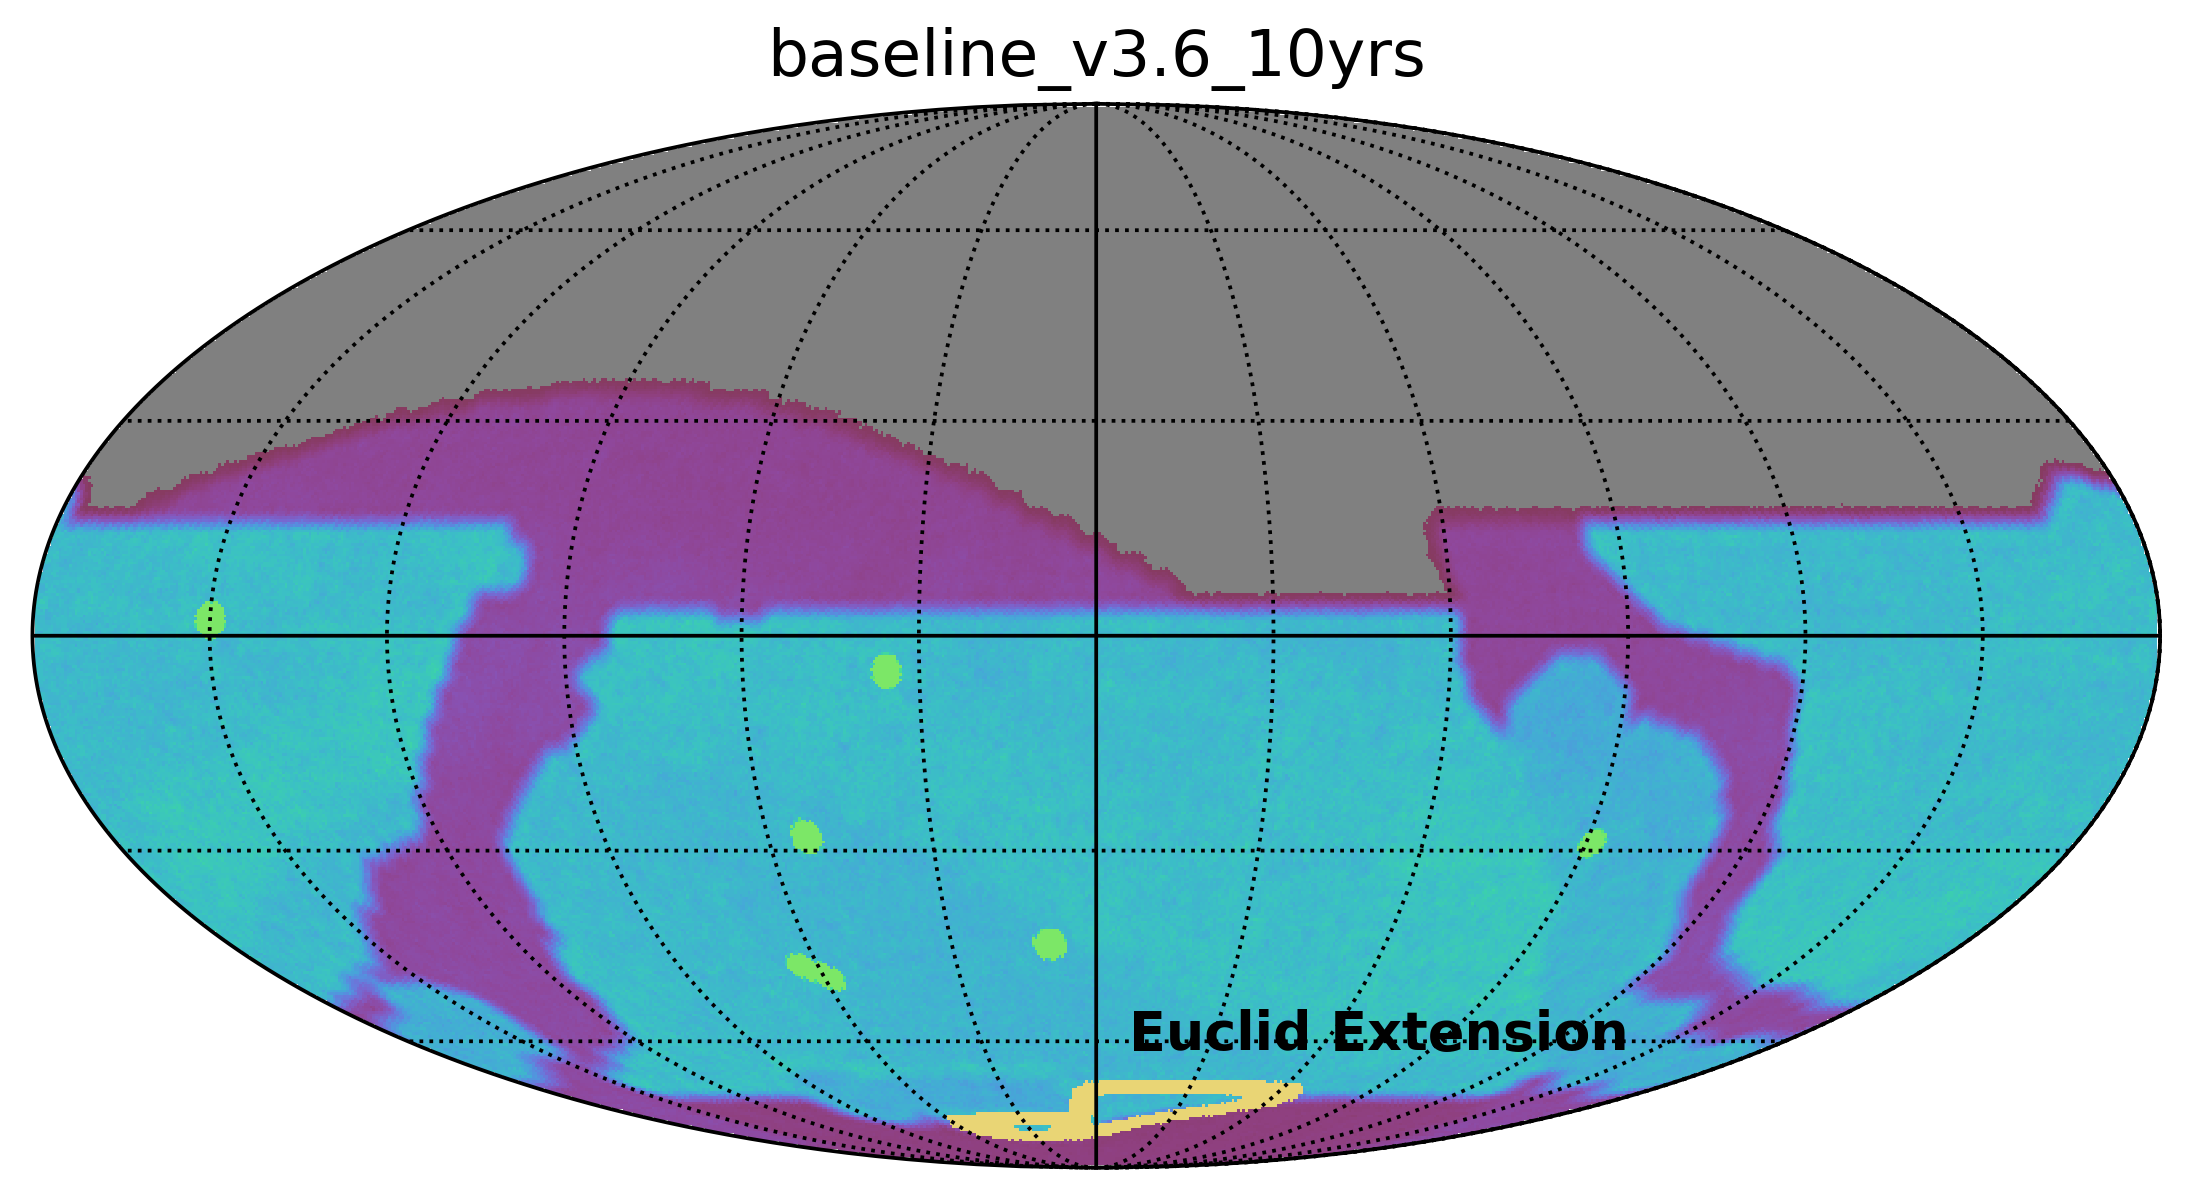
\includegraphics[width=0.45\textwidth]{figures/baseline_v3_6_10yrs_euclid_overlap.pdf}
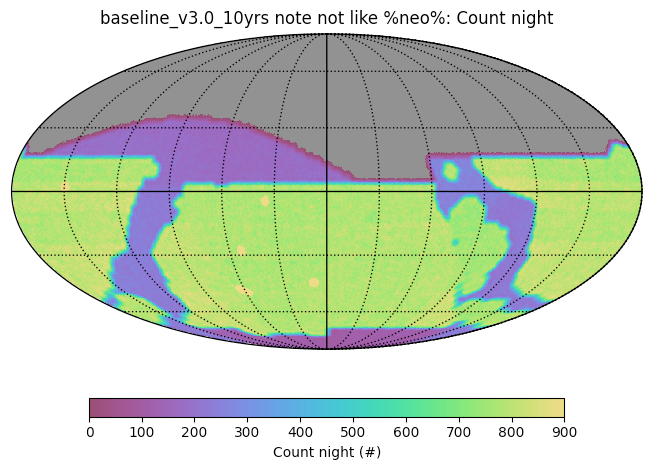
\includegraphics[width=0.45\textwidth]{figures/3.0_south.png}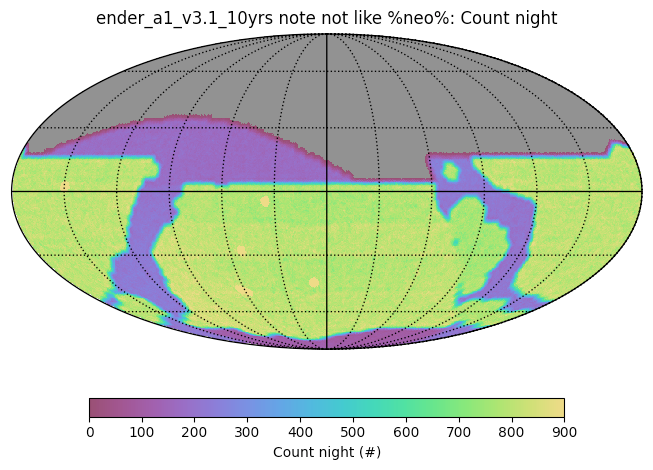
\includegraphics[width=0.45\textwidth]{figures/3.1_south.png}

\caption{Small changes to the southern portion of the footprint improve overlap with Euclid.}
\end{figure}

The airmass limits for the Near-Sun Twilight microsurvey, introduced with baseline v3.0, were increased from $X=2.5$ to $X=3.0$ in \texttt{v3.2}, corresponding with decreasing the minimum solar elongation reached for this microsurvey from 60 degrees to 45 degrees. This improves the likelihood of discovery of interior-to-earth objects, increasing the survey sensitivity to this niche of discovery space. The recovered population of objects
interior to Venus at magnitude $H\leq20$ goes from $\sim4\%$ to $\sim40\%$ in \texttt{v3.2} and later. The impacts outside the microsurvey are negligible.

\section{Additional changes introduced in \texttt{v3.6} \opsim s }\label{sec:opsimchanges}
Starting with \texttt{v3.6} some important assumptions underlying the simulations were updated: 
\begin{itemize}
\item Increased downtime in Y1 to reflect a more realistic transition into operations. The downtime in Y1 is simulated to be maximal early on and decreased to the level expected for the general LSST survey by the end of the first year. 
\item The effect of jerk on slew time is now included in the simulations, and thus included in scheduling choices.
\end{itemize}

